\documentclass[12pt]{article}
\usepackage{fullpage}
\usepackage{amsmath,amssymb,mathtools,xparse,graphicx,float}
\pagestyle{empty}
\newcommand{\D}{\displaystyle}
\setlength{\textheight}{9in} \setlength{\headheight}{.2in}
\setlength{\headsep}{0in} \setlength{\topmargin}{0in}
\begin{document}
\begin{center}
CSCI 6100 Machine Learning From Data\\
Fall 2018\\
\end{center}
\begin{center}
HOMEWORK 1\\
Daniel Southwick\\
661542908\\
southd@rpi.edu
\end{center}
\vspace{.1in}

\noindent {\bf Exercise 1.3} \\\\
\indent (a) We know that $y(t)w^T(t)x(t) < 0$, thus $x(t)$ is misclassified by $w(t)$ so $h(x)$ will always have the opposite sign comparing to the actual $y(t)$. Since $h(x) = sign(w^T(t)x(t))$ and has the opposite sign with $y(t)$, so $h(x)y(t)$ is always $>0$, thus $sign(w^T(t)x(t)y(t) > 0$ and we can conclude $y(t)w^T(t)x(t) > 0$.\\\\
\indent (b) We first move the right hand equation to the left side and we need to show: \\ $y(t)w^T(t+1)x(t) - y(t)w^T(t)x(t) > 0$. Note that $w(t+1) = w(t)+y(t)x(t)$
\begin{center}$y(t)w^T(t+1)x(t) - y(t)w^T(t)x(t)$\\$= y(t)(w^T(t+1) - w^T(t))x(t)$\\$=y(t)(w(t) + y(t)x(t) - w(t))^Tx(t)$\\$ = y(t)y(t)x^T(t)x(t)$\\$=y^2(t)x^T(t)x(t)$\\$=y^2(t)||x(t)||^2_2$
\end{center}
We know that that first element in $x(t)$ is defined as 1, so $||x(t)||^2_2 > 0$ thus $y^2(t)||x(t)||^2_2 > 0$ and $y(t)w^T(t+1)x(t) - y(t)w^T(t)x(t) > 0$ and $y(t)w^T(t+1)x(t) > y(t)w^T(t)x(t)$.\\\\
\indent (c) From part (a), $x(t)$ is correctly classified if $y(t)w^T(t)x(t) > 0$ and incorrectly classified if $y(t)w^T(t)x(t) < 0$. Either way, with the updated weight vector $w(t+1)$, $y(t)w^T(t+1)x(t) > y(t)w^T(t)x(t)$. Updated steps will always move toward positive thus in the right direction.\\\\

\noindent {\bf Exercise 1.5} \\\\
\indent Suited for the learning approach: (a), (c) and (e), the descriptive function $f$ cannot be described with data.\\
\indent Suited for the design approach: (b) and (d), the function $f$ can be directly derived from mathematical analysis.\\\\

\newpage
\noindent {\bf Exercise 1.6} \\\\
\indent (a) Recommending a book to a user in an online bookstore\\
\indent Supervised learning. We can use the store website's transaction history data and for example, group these transaction by book's categories. Within the categories we can find out the most purchased books and recommend to customers that have previously purchased some other books in the categories before.\\\\
\indent (b) Playing tic-tac-toe\\
\indent Reinforcement learning and Supervised Learning. First we can train some game's historic data of a good move of a bad move during the course of the game, we rate these data good or bad and feed into the reinforcement learning method. Second, within these good or bad action data, we can identify the best possible action throughout the game.\\\\
\indent (c) Categorizing movies into different types\\
\indent Unsupervised learning. Categorize into different types means there's no specific outcome. The data used can be the historic data of bunch of movies, and each movies are rated into different categorized such as action, comedy, horror, romance, etc.\\\\
\indent (d) Learning to play music\\
\indent Reinforcement Learning and Supervised Learning. First we can train some music's historic data on how one should play music, find out some patterns between the music notes. Second, we can train those generated music notes vs how good the music appears to be in related to human ears by the reinforcement method.\\\\
\indent (e) Credit limit\\
\indent Supervised learning. The training data can be the historic data of the debt owned and debt paid by the customers.\\\\

\noindent {\bf Exercise 1.7} \\\\
\indent (a) The picked function $g$ should be $f_8$ since $f_8$ matched with g on all three points (the most), thus $f_4$, $f_6$, $f_7$ matched with g on two points and $f_2$, $f_3$, $f_5$ matched with g on one point and $f_1$ matched with g on zero point.\\
\indent (b)The picked function $g$ should be $f_1$ since $f_1$ matched with g on zero point (the least), thus $f_2$, $f_3$, $f_5$ matched with g on two points and $f_4$, $f_6$, $f_7$ matched with g on one point and $f_8$ matched with g on zero point.(Inverse of (a))\\
\indent (c)The picked function $g$ should be $f_2$ based on XOR, thus $f_1$, $f_4$, $f_6$ matched with g on two points and $f_3$, $f_5$, $f_8$ matched with g on one point and $f_7$ matched with g on zero point.\\
\indent (d)The picked function $g$ should be $f_7$ based on XOR, thus $f_3$, $f_5$, $f_8$ matched with g on two points and $f_1$, $f_4$, $f_6$ matched with g on one point and $f_2$ matched with g on zero point. (Inverse of (c))\\

\newpage
\noindent {\bf Problem 1.1} \\\\
\indent Probability that you pick the first bag or pick the second bag are both 0.5. Suppose the 1st bag is chosen, probability of choosing black ball then is 0.5x1 = 0.5; Suppose the 2nd bag is chosen probability of choosing black ball then is 0.5x0.5 = 0.25. We add the above probability together 0.5+0.25 = 0.75, thus we get the probability that the first ball is black.\\\\
\indent Probability that both balls are black can only happens when the 1st bag is picked thus \\$P[B_2\cup B_1] = 0.5$. According to Bayes' Theorem, $P[B_2|B_1] = \frac{P[B_2\cup B_1]}{P[B_1]} = \frac{0.5}{0.75} = \frac{2}{3}$.\\

\noindent {\bf Problem 1.2} \\\\
\indent (a) Suppose the line $w_0 + w_1x_1 + w_2x_2 = 0$ that separates $h(x) = +1$ and $h(x) = -1$ exists, and we know $h(x) = sign(w^Tx)$. So $h(x)$ can only be $+1$ or $-1$. When $h(x) = +1$, $(w^Tx) > 0$, so $(x_1,x_2)$ is in the region above this line $w_0 + w_1x_1 + w_2x_2$. Similar, when $h(x) = -1$, $(x_1,x_2)$ is below the line. Thus the line exist and separate all points into two region. And: 
\begin{center}$w_0 + w_1x_1 + w_2x_2 = 0$\\$w_2x_2 = -w_0 - w_1x_1$\\$x_2 = -\frac{w_1}{w_2}x1 - \frac{w_0}{w_2}$($w_2 \neq 0$)
\end{center}
So $a = -\frac{w_1}{w_2}$ and $b = - \frac{w_0}{w_2}$\\\\
\indent (b) If $w = [1,2,3]^T$, $a = -\frac{w_1}{w_2} = -2/3$ and $b = - \frac{w_0}{w_2} = -1/3$; If $w = - [1,2,3]^T$, $a = -\frac{w_1}{w_2} = -2/3$ and $b = - \frac{w_0}{w_2} = -1/3$, same as $w = [1,2,3]^T$. So $a = -2/3$ and $b = -1/3$ (Fig \ref {fig:Pic1})
\begin{figure}[H]
  \centering
  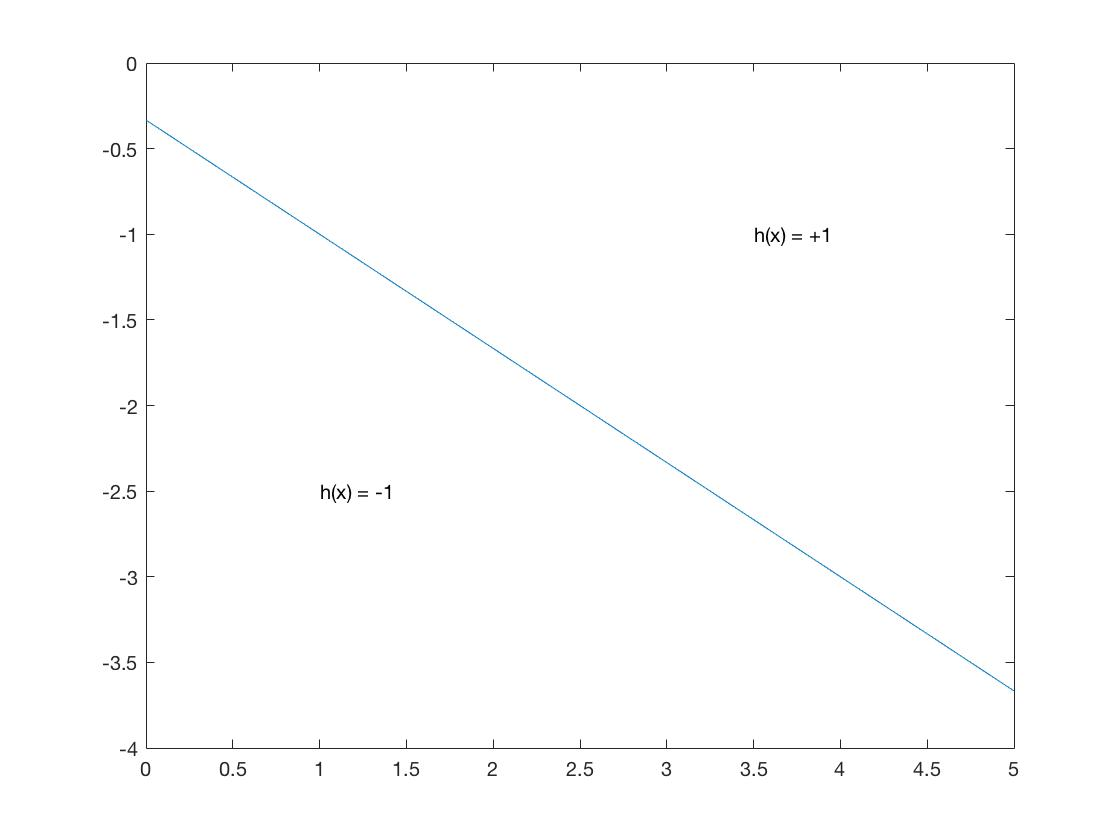
\includegraphics[scale = 0.25]{Pic1.jpg}
  \caption{Separation of H(x)}
  \label{fig:Pic1}
\end{figure}

\newpage
\noindent {\bf Problem 1.4} \\\\
\indent (a) We simply choose the target function to be $f: y=1$ with anything greater than 1 marked +1 and anything less than 1 marked -1. (Fig \ref{fig:Pic2})
\begin{figure}[H]
  \centering
  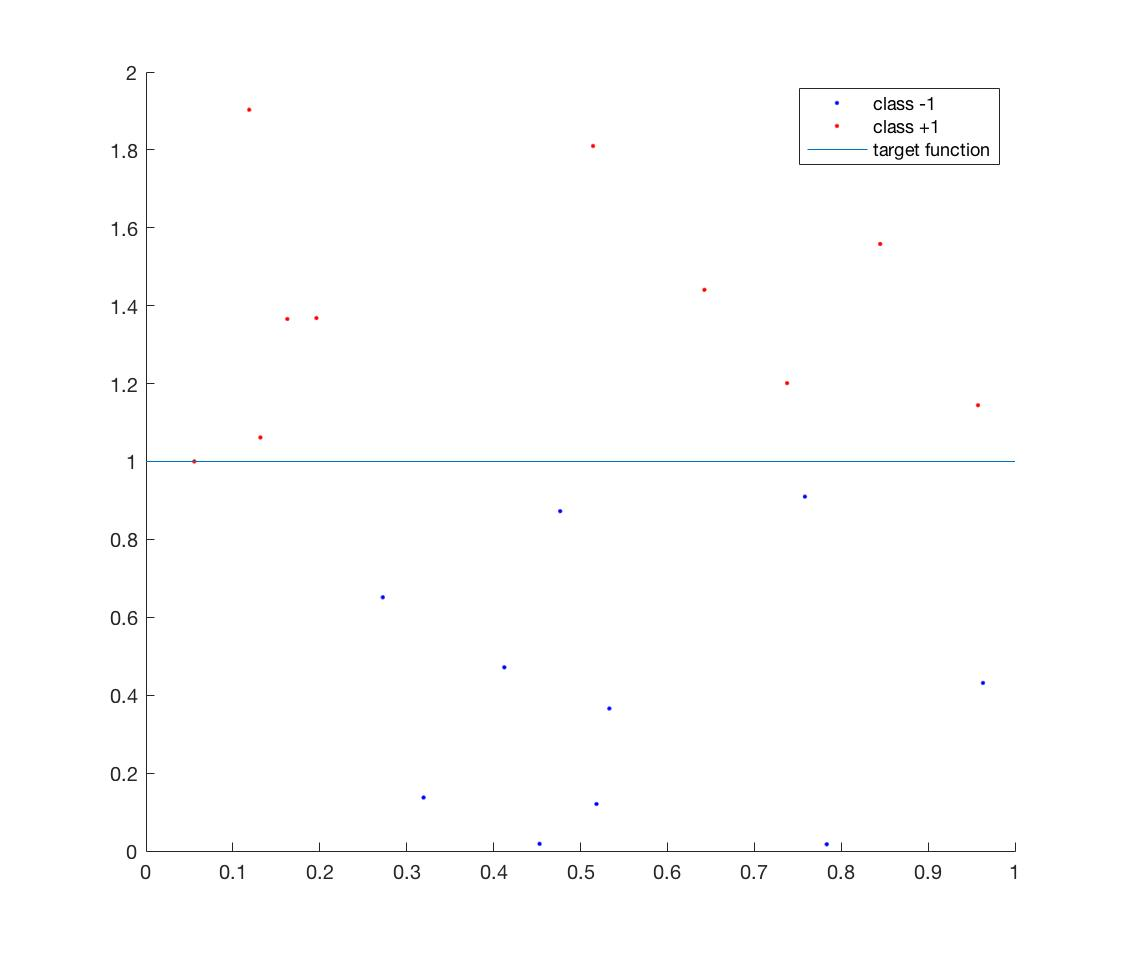
\includegraphics[scale = 0.25]{Pic2.jpg}
  \caption{Sampled example}
  \label{fig:Pic2}
\end{figure}
\indent (b) We set the initial value $w$ to be $[0.5,0.5,0.5]^T$ and the number of updates that the algorithm took before converging was 22. (Fig \ref{fig:Pic3}) We can see a clear gap between the target function $f$ and the hypothesis function $g$.
\begin{figure}[H]
  \centering
  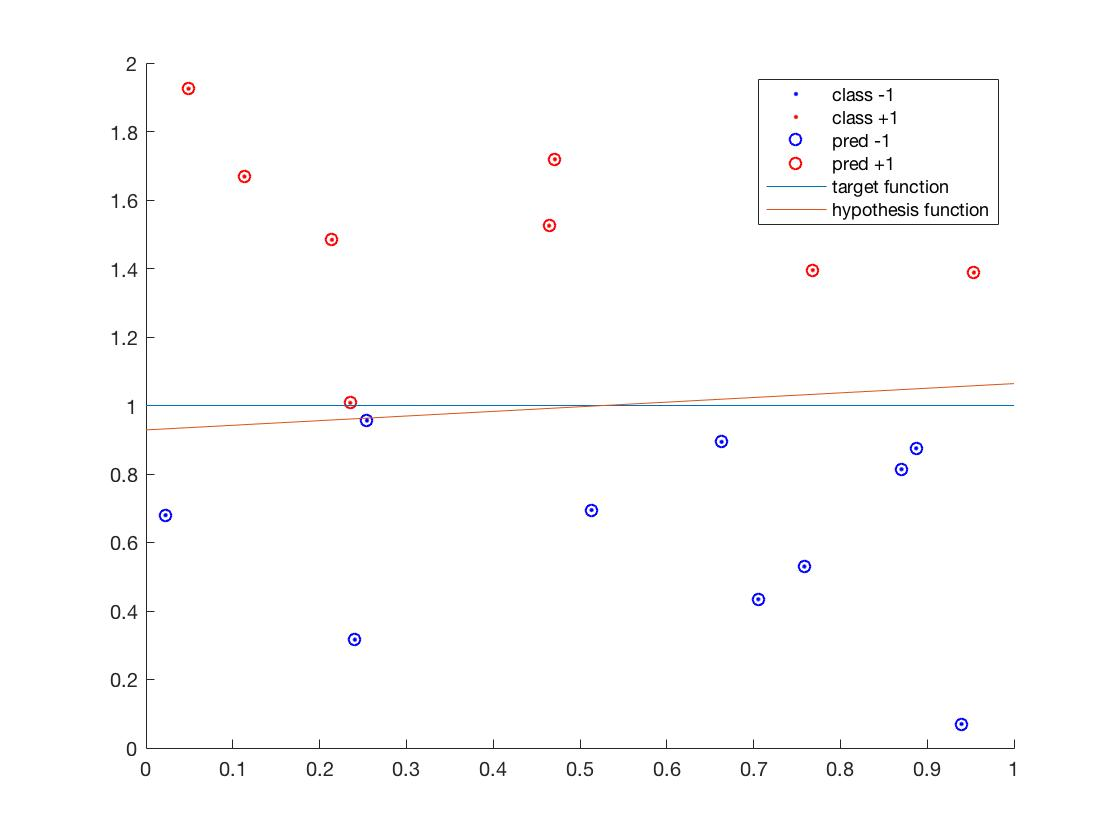
\includegraphics[scale = 0.25]{Pic3.jpg}
  \caption{Obtained function with 20 samples I}
  \label{fig:Pic3}
\end{figure}
\indent (c) We again set the initial value $w$ to be $[0.5,0.5,0.5]^T$ but use a different random data set, this time the the number of updates that the algorithm took before converging was 16. (Fig \ref{fig:Pic4}) There still exist an obvious gap between f and g and the iteration is about the same as part (b).
\begin{figure}[H]
  \centering
  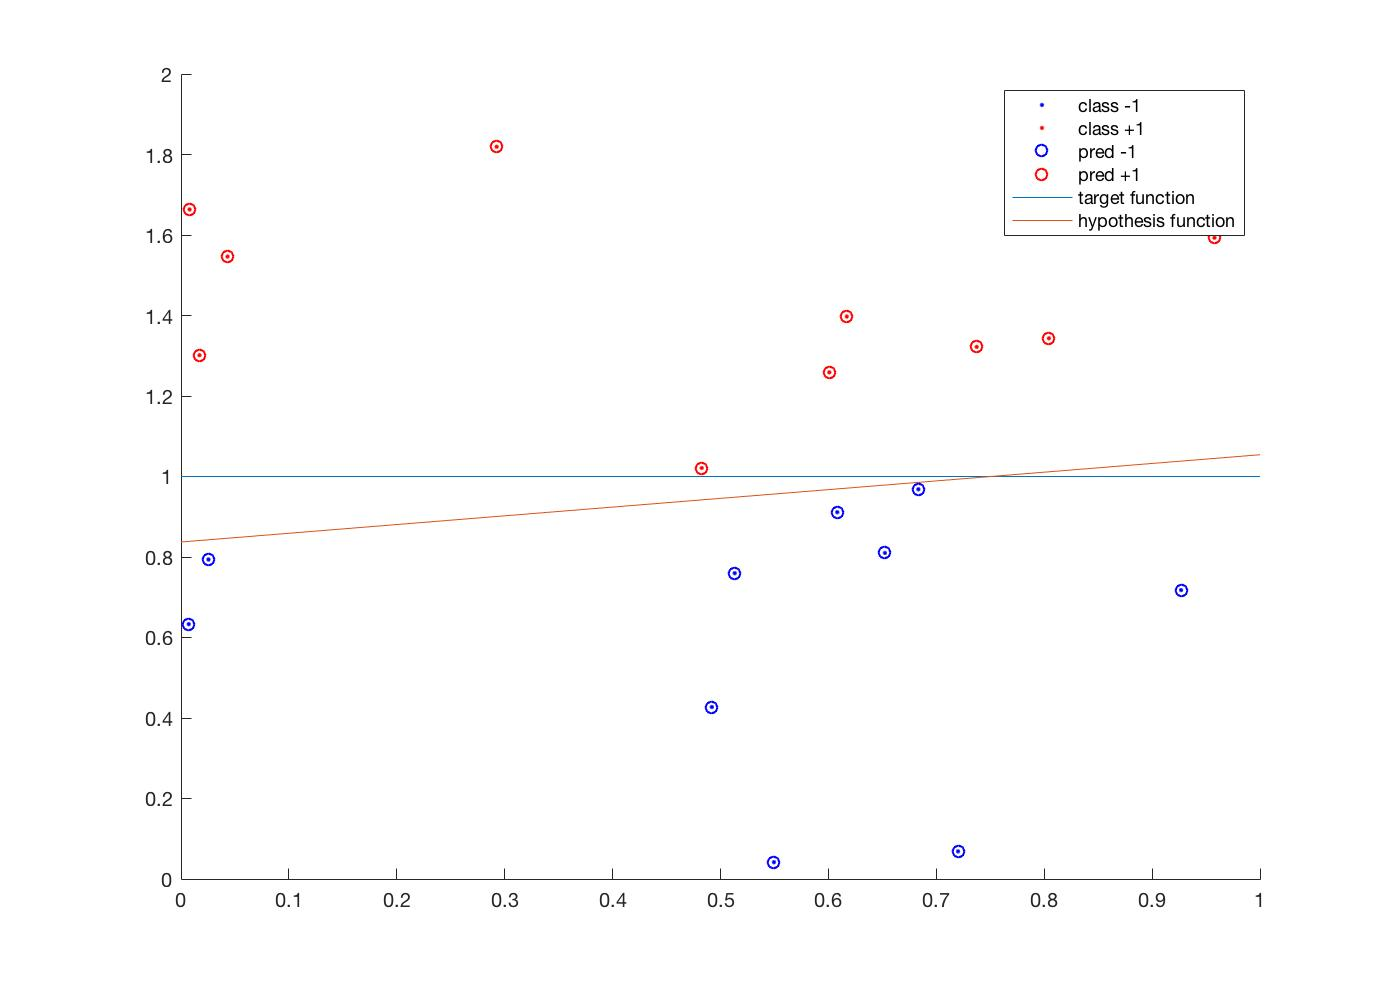
\includegraphics[scale = 0.25]{Pic4.jpg}
  \caption{Obtained function with 20 samples II}
  \label{fig:Pic4}
\end{figure}
\indent(d)Now we increase the data size from 20 to 100, again, use the same initial value $w=[0.5,0.5,0.5]^T$, this time the number of updates that the algorithm took before converging increased to 185. (Fig \ref{fig:Pic5}) The gap also became smaller but still exist compare to N = 20.
\begin{figure}[H]
  \centering
  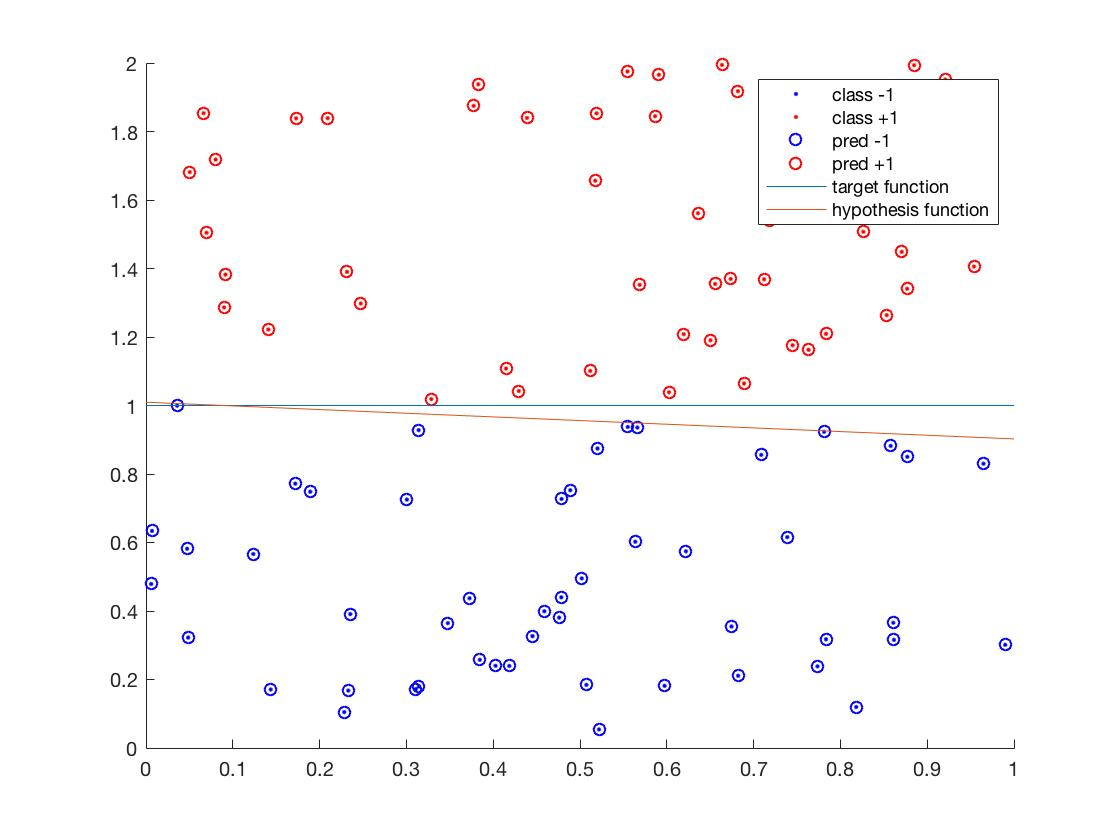
\includegraphics[scale = 0.25]{Pic5.jpg}
  \caption{Obtained function with 100 samples}
  \label{fig:Pic5}
\end{figure}
\indent(e)Now we increase the data size from to 1000, again, use the same initial value $w=[0.5,0.5,0.5]^T$, this time the number of updates that the algorithm took before converging increased to 2297. (Fig \ref{fig:Pic6}) The gap appears to disappeared compare to N=20.
\begin{figure}[H]
  \centering
  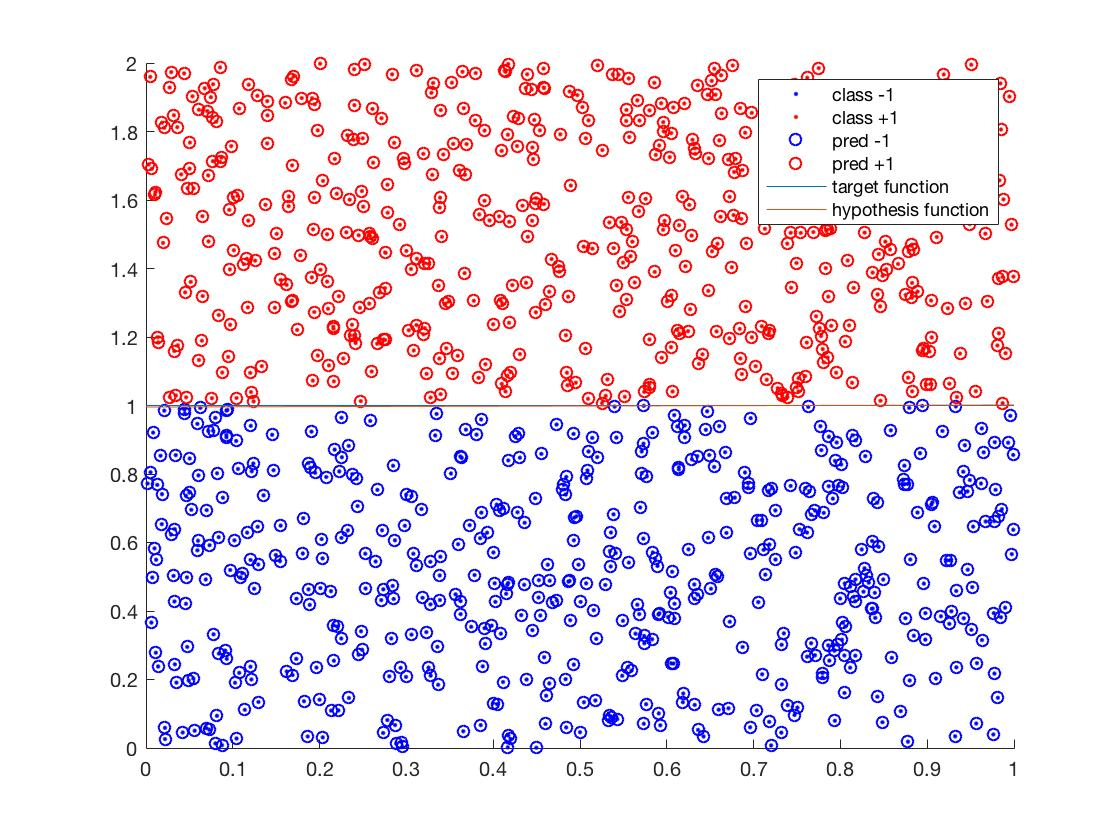
\includegraphics[scale = 0.25]{Pic6.jpg}
  \caption{Obtained function with 1000 samples}
  \label{fig:Pic6}
\end{figure}

\end{document}
